\chapter{Planejamento do Projeto}
\noindent
O desenvolvimento do projeto seguirá a sequência: primeiramente o módulo Servidor, em seguida o módulo \textit{Mobile}, e por fim o módulo BD. 

Preferiu-se utilizar tal sequência de criação para os módulos de modo a se estabelecer um modelo de processo incremental. Sobre isso, convém observar: "O modelo incremental libera uma série de versões, denominadas incrementos, que oferecem, progressivamente, maior funcionalidade ao cliente à medida que cada incremento é entregue"\cite[p. 44]{engenhariasoftware}. Assim, pode-se criar o módulo Servidor reconhecendo e detectando as faces de uma foto salva em uma pasta e exibindo o resultado (presença ou falta) na tela. Nesse sentido \citep{engenhariasoftware}, afirmam que nesse modelo de processo, geralmente, o primeiro incremento a ser produzido é um produto essencial. Isso justifica a escolha do módulo servidor como primeiro a ser desenvolvido.

Após isso, criou-se o módulo \textit{Mobile}, que envia a fotografia para o módulo Servidor. Nesse momento, o módulo 1 já desenvolvido, ao invés de procurar a fotografia em uma pasta, passa a recebê-la do módulo \textit{Mobile}, exibindo ainda as faltas na tela. A próxima etapa, será a criação do mudo BD. Ao integrar-se o módulo BD, ter-se-á faltas sendo salvas em um Banco de Dados, permitindo ainda ao módulo \textit{Mobile} a possibilidade de alterar ou consultar as mesmas. 

As semanas foram numeradas conforme a sequência no ano. Além disso, o cronograma da figura \ref{fig:figura4} apresenta na cor preta as semanas que serão dedicadas ao desenvolvimento de cada um dos tópicos. A cor cinza escura representa as semanas de Verificação Corrente e Verificação Final, elas não foram utilizadas para fins de construção do planejamento, entretanto podem ser utilizadas em último caso. A semana 26, na cor cinza mais claro, representa a 2ª semana de férias e foi utilizada para  o trabalho, porém com uma carga menor. 

\begin{figure}[!ht]
	\centering
	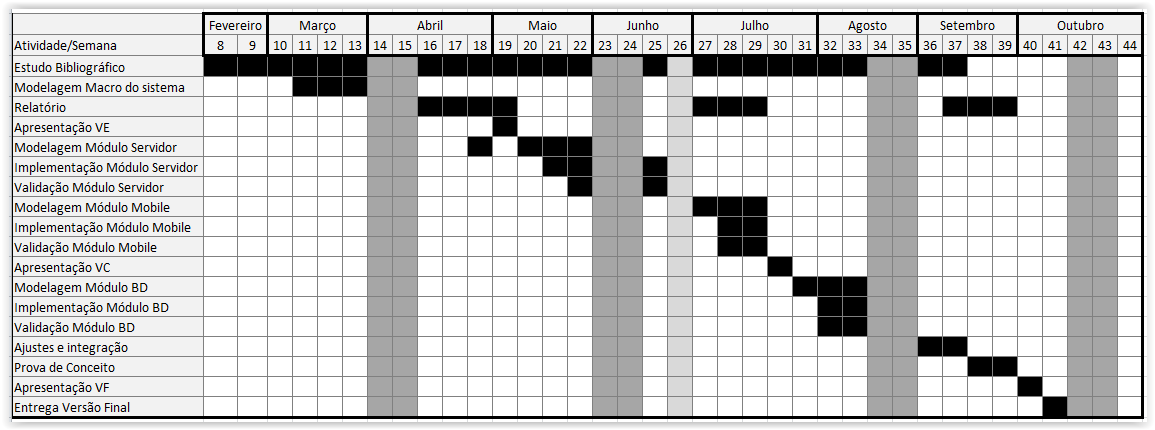
\includegraphics[width=1.0\textwidth]{cronograma.PNG}   
	\caption{Cronograma}
	\label{fig:figura5}
\end{figure}

Lista de Entregáveis:
\begin{itemize}
\item \textit{Módulo Servidor:} até o dia 18/06
\item \textit{Módulo Mobile:} até o dia 20/07
\item \textit{Módulo BD:} até o dia 17/08
\item \textit{Prova de conceito:} até o dia 28/09
\end{itemize}


